\documentclass{beamer}

\setlength{\parskip}{\baselineskip}
\setlength{\parindent}{0pt}
\usepackage{default}
\usepackage{tabularx}
\usepackage{url}
\usepackage{graphicx}
\usepackage{listings}
\usepackage{color}
\usepackage{amssymb,amsmath,amsthm,mathrsfs,mathtools,amscd}
\usepackage{mathrsfs}

\definecolor{darkgreen}{rgb}{0,0.6,0}
\definecolor{lightblue}{rgb}{0.10,0.85,1.0}
\definecolor{darkgreen}{rgb}{0,0.6,0}
\definecolor{tudblue}{rgb}{.004,.50,.78} % definition TUDelft blue color
\definecolor{tudlightblue}{rgb}{.004,.70,.98}

\newenvironment{recap}{\begin{small}\color{gray}\begin{flushright}}{\end{flushright}\end{small}}


\title{\huge{Citation Management with \texttt{JabRef}}}
\author{\textbf{Manuel Baumann}, Jan Heiland}
\titlegraphic{
   \includegraphics[scale=0.08]{images/TU_Delft_logo1.png}\hspace{4cm}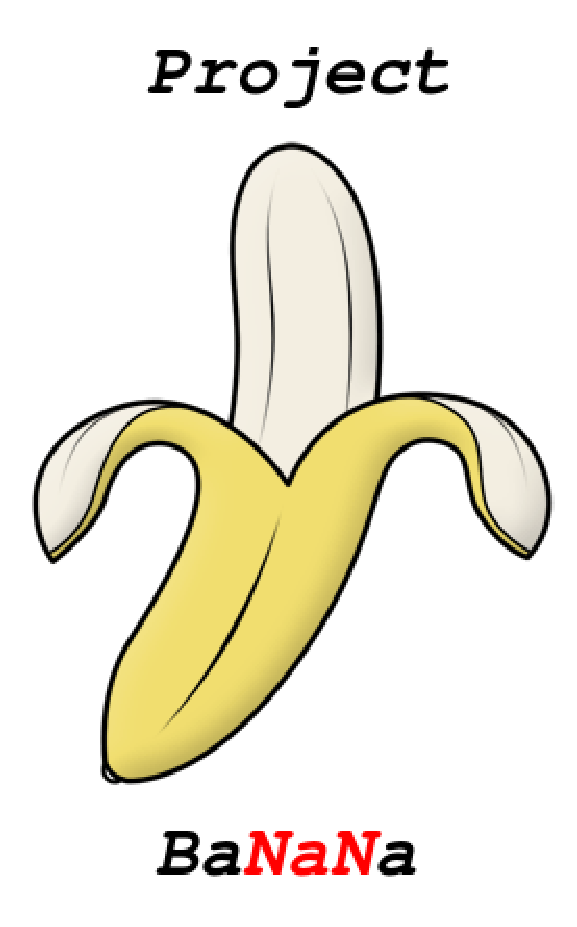
\includegraphics[scale=0.15]{../../images/logo}}
\date{\footnotesize{December 19, 2013}}

\begin{document}

\frame{\titlepage}

\begin{frame}[fragile]
\frametitle{\LaTeX \ and bib-files}
How bibtex is used in \LaTeX:
\vspace{1cm}
\begin{small}
\lstset{language=[LaTeX]TeX,
texcsstyle=*\bf\color{blue},
numbers=none,
breaklines=true,
keywordstyle=\color{darkgreen},
commentstyle=\color{darkgreen},
frame=none,
tabsize=2}
\begin{lstlisting}
\documentclass{article}
\usepackage{hyperref}	    % very fancy; else:'cite'

\begin{document}

See, \cite{Saad93}.       % cite a reference

\bibliography{my_bib}     % use file 'my_bib.bib'
\bibliographystyle{plain}

\end{document}
\end{lstlisting}
\end{small}
\end{frame}

\begin{frame}[fragile]
A bibtex file is a plain text file with entries of this type:
\vspace{0.7cm}
\begin{footnotesize}
\lstset{language=[LaTeX]TeX,
escapeinside={(*@}{@*)},
texcsstyle=*\bf\color{blue},
numbers=none,
breaklines=true,
keywordstyle=\color{blue},
morekeywords={*,@ARTICLE},
frame=none,
tabsize=2,
emph={author, title, journal, year, volume, pages, file, owner, timestamp},
emphstyle={\color{tudblue}}
}
\begin{lstlisting}
@ARTICLE{(*@\color{darkgreen}Saad93@*),
  author    = {Y. Saad},
  title     = {A flexible inner-outer preconditioned            {GMRES} algorithm},
  journal   = {SIAM J. Sci. Comput.},
  year      = {1993},
  volume    = {14},
  pages     = {461-469},
  file      = {:Literature/Saad_flexibleGMRES.pdf:PDF},
  owner     = {manuel},
  timestamp = {2013.09.09}
}
\end{lstlisting}
\end{footnotesize}
\end{frame}

\begin{frame}
\frametitle{What is \texttt{JabRef}?}
\framesubtitle{Basic Functionality}
\vspace{0.6cm}\\
The tool \texttt{Jabref} \ldots \\
\begin{itemize}
\item \ldots is GPL software 
\item \ldots comes for all platforms
\item \url{http://sourceforge.net/projects/jabref/}
\end{itemize}
\vspace{0.5cm}\\
Moreover, \texttt{Jabref} can\\
\begin{itemize}
\item open several bibs in a GUI
\item sort them by author, title, year, etc.
%\item copy and paste between the libs
\item edit the entries
\item assign files like PDFs to the entries
\item auto-generate citation keys \texttt{[author][year]}
\end{itemize}\\
\hfill $\hookrightarrow$ live performance
\end{frame}

\begin{frame}
\frametitle{What is \texttt{JabRef}?}
\framesubtitle{Import/Export of bibtex entries}
Importing of bibtex entries:
\begin{itemize}
 \item via copy-n-paste from other bib-files
 \item from plain text
 \item from the Internet
\end{itemize}

Interplay with the Latex Editor:
\begin{itemize}
 \item ctrl-K copies  ``$\backslash$cite$\{$citationKey$\}$`` to the clipboard
\end{itemize}
\vfill
\hfill
$\hookrightarrow$live performance
\end{frame}

\begin{frame}
\frametitle{Set up \texttt{JabRef} on our machines...}
Unfortunatelly, \texttt{JabRef} is not pre-installed on our workstations. 

However, this is how you can manually install it:
\begin{enumerate}
 \item Note that \texttt{JabRef} itself is a Java program
 \item Go to \url{http://jabref.sourceforge.net/download.php}
 \item Download \texttt{JabRef.jar}
 \item Type in the terminal: \texttt{java -jar JabRef.jar}
 \item If you want, define the terminal command \texttt{'jabref'} in your \texttt{/.local/bin}
 \pause
 \item Or, simply ask Joost
\end{enumerate}
\pause
Maybe, don't start with step \color{blue}6.\color{black}
\end{frame}

\begin{frame}
\frametitle{Citations in Math-Manuscripts}
\framesubtitle{Some general remarks...}
Bibtex entries are provided by most of the services that list or host scientific papers. In particular for mathematics it may be worth checking
\begin{itemize}
\item \url{http://www.ams.org/mathscinet/index.html}
\item \url{http://www.zentralblatt-math.org/zmath/en/search/} ( features a ``TU'' button )
\item \url{http://www.sciencedirect.com/}
\item and also most of the preprint servers 
\end{itemize}
Q: How do you do it?
\end{frame}


\begin{frame}
\frametitle{Further reading}
Many information are available online:
\begin{itemize}
 \item \url{http://www.cs.rpi.edu/~tayloj/JABREF.TUTORIAL/}
 \item \url{http://www.youtube.com/watch?v=_bdmCi58o74}
 \item \small{\url{http://keijisaito.info/arc/biblio/en_jabref_bibtex.htm}}
\end{itemize}
I will put all example files on:
\begin{itemize}
 \item \url{http://projectbanana.github.io/}
\end{itemize}
 \begin{figure}
\centering
 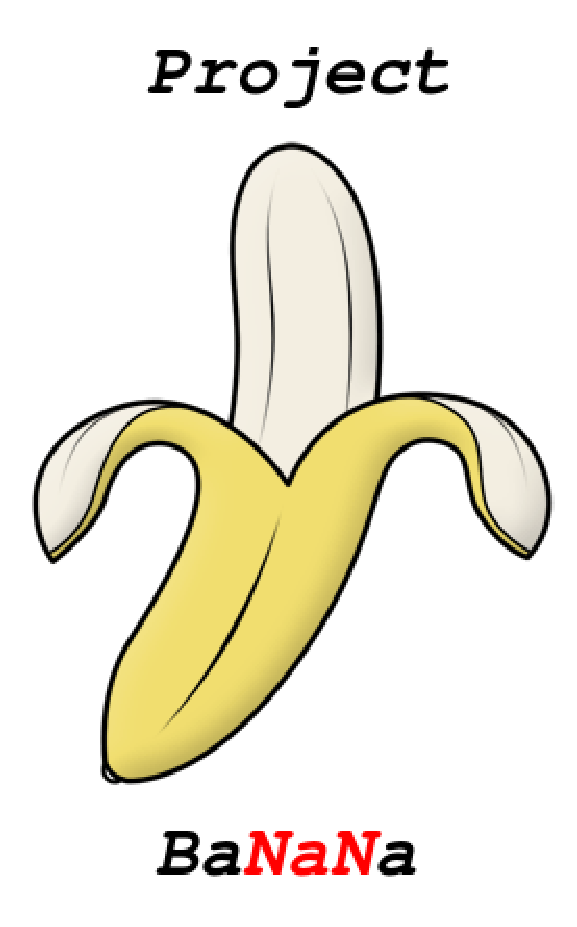
\includegraphics[height=0.3\textheight]{../../images/logo}
\end{figure}
\end{frame}

\end{document}
